\section{Floating point}

A finite set of machine numbers, denoted as $\mathbb{F}=\{-\tilde{a}_{min},\dots,\tilde{a}_{max}\}$ and referred to as floating-point numbers, is employed by calculators due to their limited capacity to store numbers and perform operations.
The process of mapping a real number from the set $\mathbb{R}$ to a value in $\mathbb{F}$ is achieved using the function $fl(x)$, which involves both truncation and rounding operations.

The set $\mathbb{F}=\mathbb{F}(\beta,t,L,U)$ is defined by four parameters: $\beta,t,L$ and $U$. 
These parameters collectively characterize every real number $fl(x) \in \mathbb{F}$, which can be expressed as:
\[fl(x)=(-1)^s(0.a_1a_2\dots a_t)\beta^e\]
Here's what each component represents:
\begin{itemize}
    \item $\beta \geq 2$ is the base, an integer determining  the numeric system. 
    \item $m=(0.a_1a_2\dots a_t)$ represents the mantissa.
    \item $e \in \mathbb{Z}$ is the exponent, subject to the constraints $L<e<U$, with $L<0$ and $U>0$. 
    \item $s=\{0,1\}$ denotes the sign.
\end{itemize}
In defining the numbers in the mantissa set, a crucial condition is that $a_1 \neq 0$ to ensure the uniqueness of the representation. 
In such cases, the number is referred to as normalized.

The set of floating-point numbers exhibits several characteristic values and properties:
\begin{itemize}
    \item Machine epsilon: it represents the gap between 1 and the smallest floating-point number greater than 1, and it is given by the formula:
        \[\varepsilon_M=\beta^{1-t}\]
    \item Round-off error: this error reflects the relative error introduced when replacing a real number $x \in \mathbb{R}-\{0\}$ with its corresponding $fl(x) \in \mathbb{F}$. 
        It is bounded by the condition:
        \[\dfrac{\left\lvert x-fl(x) \right\rvert}{\left\lvert x \right\rvert }\leq \dfrac{1}{2}\varepsilon_M\]
        where $x \neq 0$.
    \item The biggest and the smallest numbers in the set: these can be calculated using the following formulas:
        \[x_{min}=\beta^{L-1}\]
        \[x_{max}=\beta^U(1-\beta^{-t})\]
\end{itemize}
\begin{example}
    In MATLAB, the floating-point set is defined with the following parameters:
    \[(\beta=2,t=53,L=-1021,U=1024)\] 
    With the command "eps" we can find the machine epsilon, that in MATLAB case is:
    \[\epsilon_M=2.22 \cdot 10^{-16}\]
    With the command "realmin" and "realmax" we can find the smallest and the largest numbers representable that are equal to:
    \[x_{min}=2.225073858507201 \cdot 10^{-308}\]
    \[x_{max}=1.797693134862316 \cdot 10^{308}\]
\end{example}
An important observation is that not all real numbers are representable in the floating-point set, resulting in a lack of continuity in the latter. 
Increasing the magnitude of numbers in $\mathbb{R}$ also leads to an increase in the gap between consecutive numbers in $\mathbb{F}$. 
\begin{example}
    Let us consider the floating number set $\mathbb{F}(2,2,-1,2)$. 
    The characteristic values of this set are: 
    \begin{itemize}
        \item $\epsilon_M=\beta^{1-t}=0.5$.
        \item $x_{min}=\beta^{L-1}=0.25$.
        \item $x_{max}=\beta^U(1-\beta^t)=3$.
        \item $\#\mathbb{F}=2 \beta^{t-1}(\beta -1)(U-L+1)+1=16$. 
    \end{itemize}
    The exponent can take values of $-1,0,1$ and $2$, and the mantissa is represented as $(a_1a_2)_{\beta}$ due to $t=2$. 
    A figure illustrates the possible positive values in this set.
    \begin{figure}[H]
        \centering
        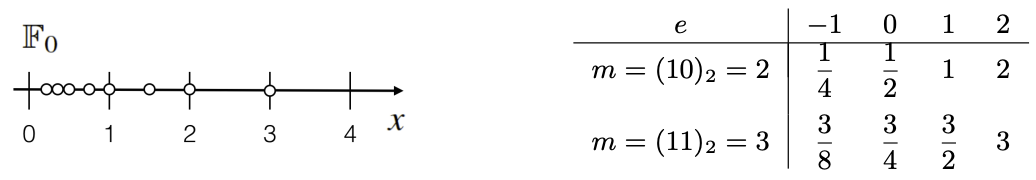
\includegraphics[width=0.9\linewidth]{images/numbers.png}
    \end{figure}
\end{example}
One notable consequence of transitioning between the two sets ($\mathbb{R}$ and $\mathbb{F}$) is the loss of two essential properties: associativity and the neutral element for addition.